In this section, we will explain our findings of different buildings from the perspective of supply and demand analysis. We have completed the analysis for the following buildings where there is a high supply-demand problem:
\begin{itemize}
    \item Redmond Building, Parkville (115) - Appendix Table \ref{appendix:red_tr}
    \item The Spot Building, Parkville (110) - Appendix Table \ref{appendix:spot}
    \item Glyn Davis Building, Parkville (133) - Appendix Table \ref{appendix:glyn}
    \item Old Arts Building, Parkville (149) - Appendix Table \ref{appendix:old}
    \item Medical Building, Parkville (181) - Appendix Table \ref{appendix:med}
    \item The Ian Potter South Bank Centre Building, Southbank  (880) - Appendix Table \ref{appendix:sth-ian}
    \item Werribee Pathology Building, Werribee (416) - Appendix Table \ref{appendix:wer-path}
\end{itemize}

We will be summarising results for \texttt{Redmond Barry Building}, \texttt{The Spot Building}, \texttt{Ian Potter Centre Building} and \texttt{Werribee Pathology Building}as discussed in the below section.


\paragraph{ Redmond Barry Building (Parkville Campus)}
\begin{figure}[H]
\centering
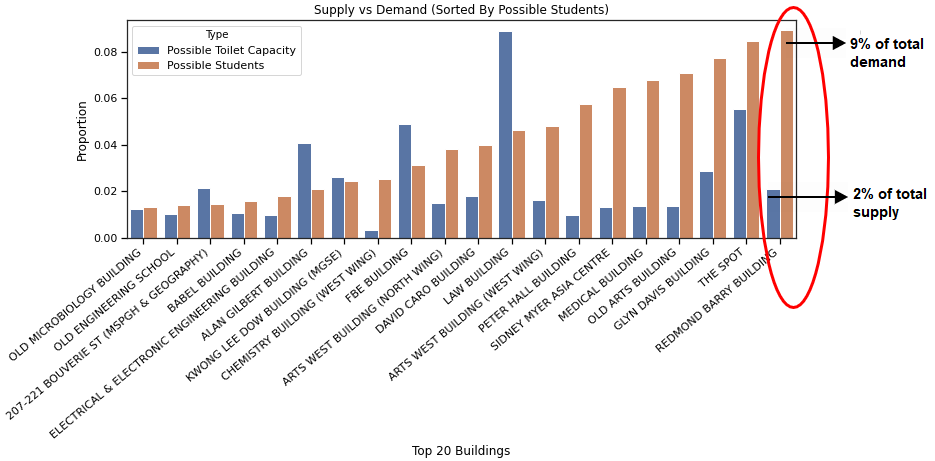
\includegraphics[width=10cm,keepaspectratio=true]{resources/images/spatial-tr/redmond2.PNG}
\caption{Supply vs Demand Problem in Redmond Barry Building}
\label{fig:eedmond_mr_s_vs_d}
\end{figure}

From the above plot, it can be seen that there is a high chance the students might not be able to find toilet facilities in the mentioned building. Hence, by using the proposed algorithm, we find the nearest building from Redmond Barry building based on the different factors as explained below.
\begin{itemize}
    \item \textbf{Best nearby buildings with no preference:}
    As given in the appendix Table \ref{appendix:red_tr}, a student needs to walk at least \texttt{422} meters from Redmond Barry Building to use the toilet facilities with an adequate supply of the mentioned facilities. The results also suggest a relaxing parameter ($\delta$) of \texttt{186.24} meters so that the students can do not miss out on a highly rewarding building. Using these constraints, it suggests that \texttt{OLD PHYSICS BUILDING (128)}  the most rewarding building with the cost of \texttt{189.14} meters as shown in Figure \ref{fig:red}. 
    % followed by \texttt{Baldwin Spencer Building (113)} with cost \texttt{11.78} meters and followed by \texttt{Old Quadrangle Building (150), Elisabeth Murdoch Building (134),David Caro Building} with cost \texttt{182.72,122.74,103.28} meters respectively, 
    
\begin{figure}[H]
\begin{subfigure}{.5\textwidth}
\centering
  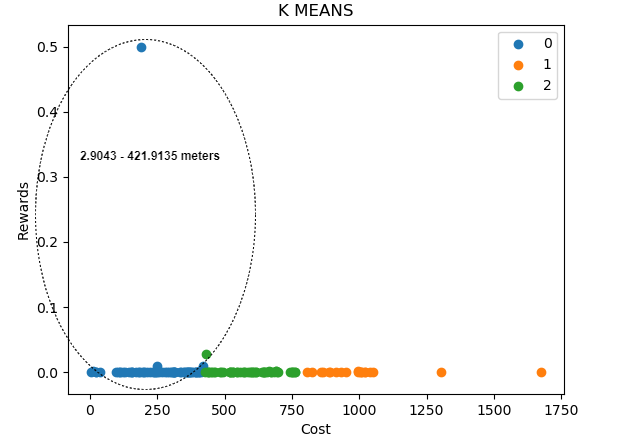
\includegraphics[width=8cm]{resources/images/spatial-tr/115plot.png}
\end{subfigure}%
\begin{subfigure}{.5\textwidth}
  \centering
  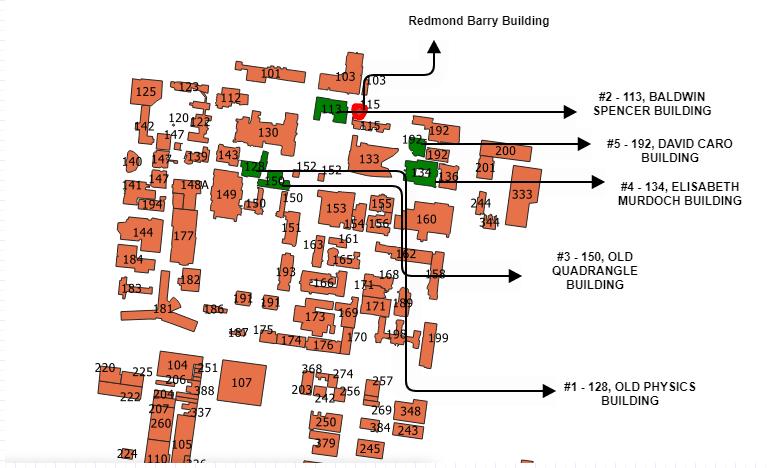
\includegraphics[width=8cm]{resources/images/spatial-tr/red1.PNG}
\end{subfigure}
\caption{Best rewarding cluster (left) and 3 most optimal buildings from Redmond Barry Building (right)}
\label{fig:red}
\end{figure}
% \item \textbf{Best nearby buildings under COVID-19 Strict Lockdown:} As given in the appendix Table \ref{appendix:red_tr} with COVID-19 strict factor, a student should be willing to walk \texttt{806.4439} meters from the mentioned building to be able to get to the buildings having adequate supply of toilet facilities. A relaxation parameter ($\delta$) of \texttt{16.31} meters could help a student to find a high rewarding building. Using the results mentioned in the table, it is seen that \texttt{The Law Building (106)} has the highest reward with \texttt{822.75} meters as the cost, followed by \texttt{The Spot (110), The FBE (105), Alan Gilbert(104) , Glyn Davis buildings(133)} respectively with costs \texttt{753.73,684.47,572.46,36.44} meters.

\item \textbf{Best nearby buildings with Good Toilet Room Conditions:}
In the appendix Table \ref{appendix:red_tr}, we have room condition as one of the factors with its budget and relaxing budgets. Using this data, we suggest that a student should walk at least \texttt{2.9043} meters to get to the rewarding building and the relaxing parameter would get a student to an even more rewarding building if a student decides to walk \texttt{186.24} meters from the current building. The most rewarding building is \texttt{Old Physics Building (128)} and followed by \texttt{Baldwin Spencer (113), David Caro (192) buildings} in order with costs \texttt{11.78,103.28,96.91,144.02} meters.

\item \textbf{Best nearby buildings with other factors:} In the appendix Table \ref{appendix:red_tr}, we have also shown other factors such as finding toilet rooms with high capacity, strict covid-19 lockdown, and easy availability with their budgets and relaxing budgets. Using those constraints, we suggest that \texttt{Old Physics Building (128) - 189.14 meters} is the most rewarding building for toilets with high capacity and for finding toilets which are easily available and using the results mentioned in the table, it is seen that \texttt{ The Law Building(106) } has the highest reward with \texttt{822.75} meters as the cost.

The results of some of the above-discussed factors are summarized below using clustering diagrams.
\end{itemize}

\begin{figure}[H]
\centering
\begin{subfigure}[b]{0.30\textwidth}
  \centering
  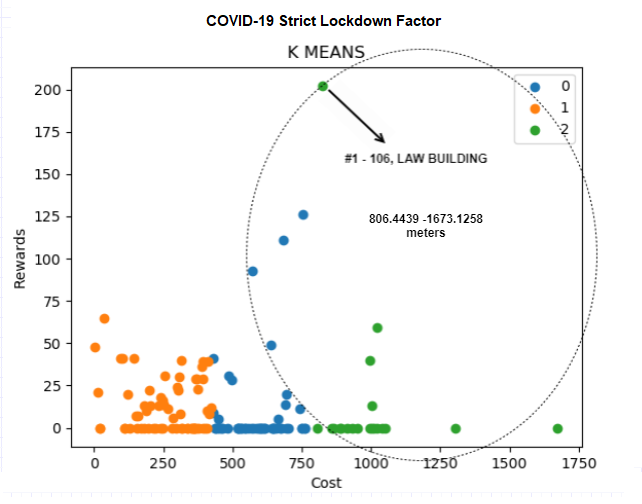
\includegraphics[width=5.5cm,keepaspectratio=true]{resources/images/spatial-tr/115_covidplot.png}
\end{subfigure}
\begin{subfigure}[b]{0.30\textwidth}
  \centering
  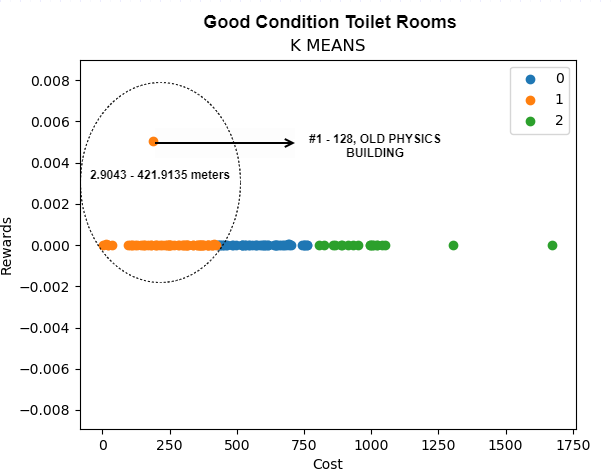
\includegraphics[width=5.5cm,keepaspectratio=true]{resources/images/spatial-tr/115_goodplot.png}
\end{subfigure}
\begin{subfigure}[b]{0.30\textwidth}
  \centering
  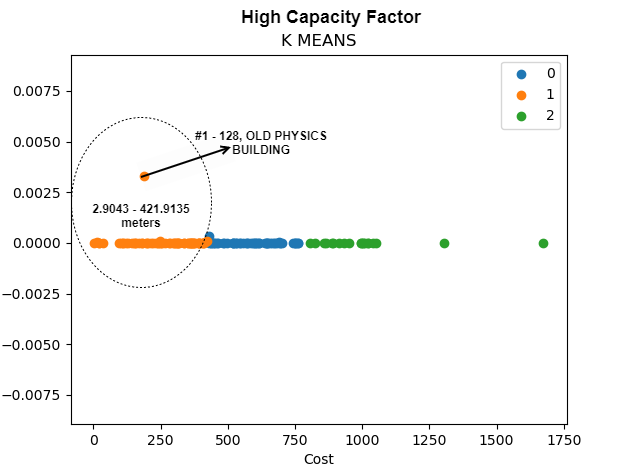
\includegraphics[width=5.5cm,keepaspectratio=true]{resources/images/spatial-tr/115_highplot.png}
\end{subfigure}
\caption{Best rewarding clusters of nearby buildings from Redmond Barry Building based on different factors}
\label{fig:redmond_factors}
\end{figure}

% \paragraph{Glyn Davis Building (Parkville Campus)}
% \begin{figure}[H]
% \centering
% 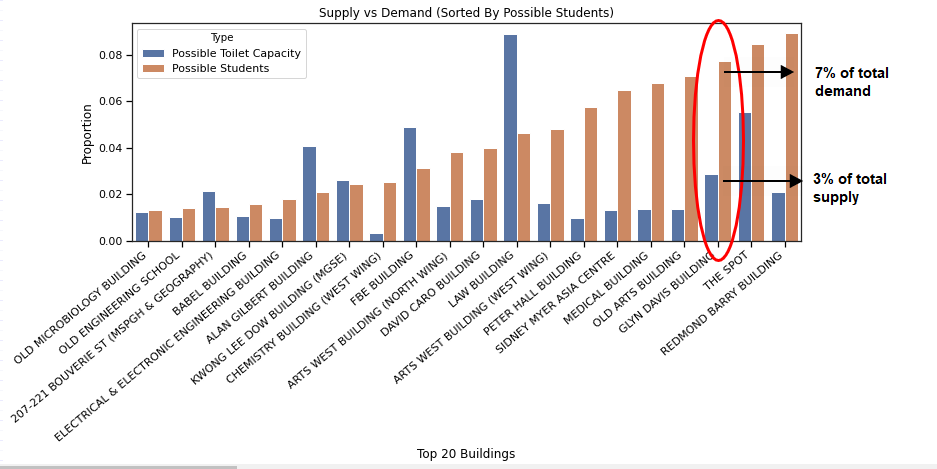
\includegraphics[width=10cm,keepaspectratio=true]{resources/images/spatial-tr/glyn.PNG}
% \caption{Supply vs Demand Problem in Glyn Davis Building}
% \label{fig:glyn}
% \end{figure}
% \begin{itemize}
%     \item \textbf{Best nearby buildings with no preference:}
%     As given in the appendix Table \ref{appendix:glyn}, a student needs to walk just \texttt{13.2} meters from Glyn Davis Building to use the toilet facilities with an adequate supply of the mentioned facilities. The results also suggest a relaxing parameter ($\delta$) of \texttt{147.10} meters so that the students can do not miss out on a high rewarding building. Using these constraints,it suggest that \texttt{OLD PHYSICS BUILDING (128)} is the most rewarding building with the cost of \texttt{160.33} meters followed by \texttt{Walter Boas Building (163)} with cost \texttt{140.22} meters and followed by \texttt{Baldwin Spencer (113), Alice Hoy Building (162),Old Quadrangle (150)} Buildings with cost \texttt{27.19,131.2,118.59} meters respectively, as shown in Figure \ref{fig:g}
    
% \begin{figure}[H]
% \begin{subfigure}{.5\textwidth}
% \centering
%   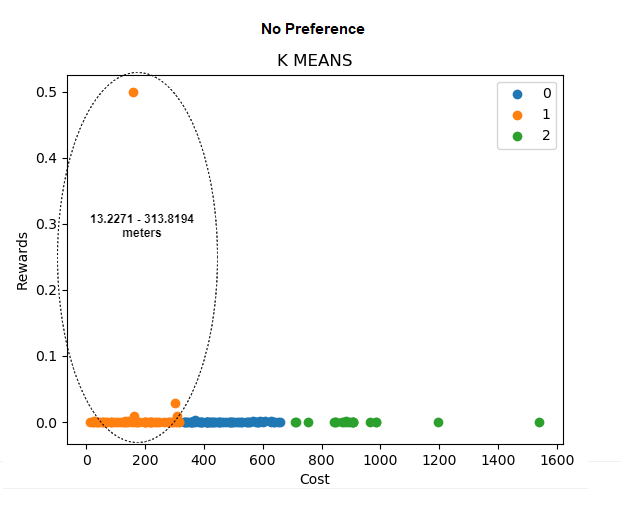
\includegraphics[width=8cm]{resources/images/spatial-tr/133plot.png}
% \end{subfigure}%
% \begin{subfigure}{.5\textwidth}
%   \centering
%   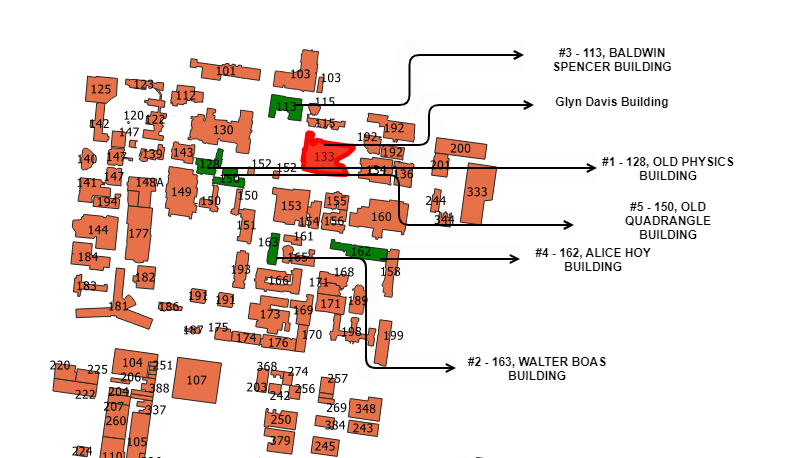
\includegraphics[width=8cm]{resources/images/spatial-tr/glyn1.PNG}
% \end{subfigure}
% \caption{Best rewarding cluster (left) and 3 most optimal buildings from Glyn Davis Building (right)}
% \label{fig:g}
% \end{figure}
    
%     \item \textbf{Best nearby buildings under COVID-19 Strict Lockdown:} As given in the appendix Table \ref{appendix:glyn} with COVID-19 strict factor, a student should be willing to walk \texttt{709.65} meters from the mentioned building to be able to get to the buildings having an adequate supply of toilet facilities. A relaxation parameter ($\delta$) of \texttt{4.96} meters could help a student to find a high rewarding building. Using the results mentioned in the table, it is seen that \texttt{The Law Building (106)} has the highest reward with \texttt{822.75} meters as the cost, followed by \texttt{The Spot (110), The FBE (105), Alan Gilbert(104) , Glyn Davis buildings(133)} respectively with costs \texttt{653.57,583.11,475.22,524.4} meters
    
%     \item \textbf{Best nearby buildings with Good Toilet Room Conditions:}
% In the appendix Table \ref{appendix:glyn},we have Room condition as one of the factors with its budget and relaxing budgets. Using this data, we suggest that a student should walk at least \texttt{13.22} meters to get to the rewarding building and the relaxing parameter would get a student to an even more rewarding building if a students decides to walk \texttt{147.1} meters from the current building.The most rewarding building is \texttt{Old Physics Building (128)} and followed by \texttt{Baldwin Spencer (113), David Caro (192) buildings} in order with costs \texttt{27.19,22.08,57.2,56.65} meters.

% \item \textbf{Best nearby buildings with other factors:} In the appendix Table \ref{appendix:glyn}, we have also shown other factors such as finding toilet rooms with high capacity,and easy availability with their budgets and relaxing budgets. Using those constraints, we suggest that \texttt{Old Physics Building (128) - 160.33 metres} is the most rewarding building for toilets with high capacity and for finding toilets which are easily available.

% The results of some of the above discussed factors are summarized below using clustering diagrams.
% \end{itemize}

% \begin{figure}[H]
% \centering
% \begin{subfigure}[b]{0.30\textwidth}
%   \centering
%   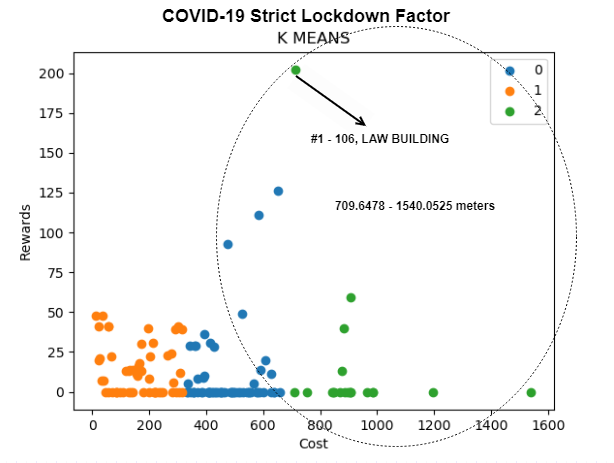
\includegraphics[width=5.5cm,keepaspectratio=true]{resources/images/spatial-tr/133_covidplot.png}
% \end{subfigure}
% \begin{subfigure}[b]{0.30\textwidth}
%   \centering
%   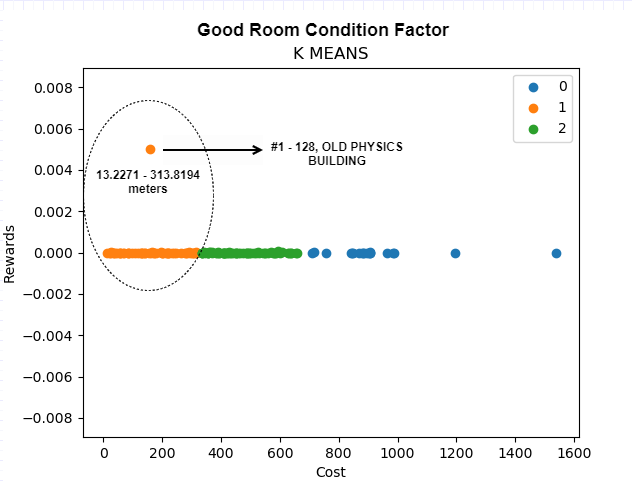
\includegraphics[width=5.5cm,keepaspectratio=true]{resources/images/spatial-tr/133_roomplot.png}
% \end{subfigure}
% \begin{subfigure}[b]{0.30\textwidth}
%   \centering
%   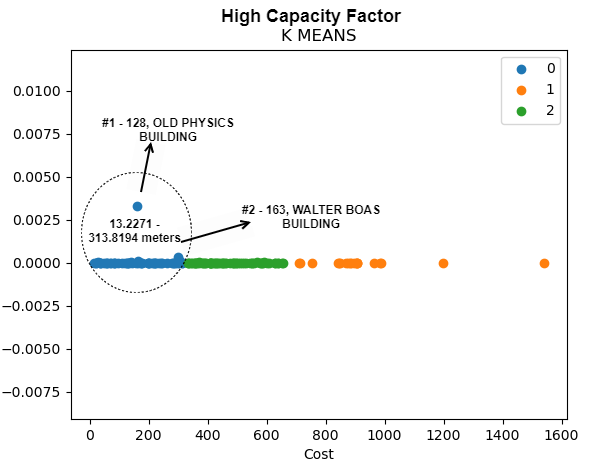
\includegraphics[width=5.5cm,keepaspectratio=true]{resources/images/spatial-tr/133_highplot.png}
% \end{subfigure}
% \caption{Best rewarding clusters of nearby buildings from Glyn Davis Building based on different factors}
% \label{fig:glyn_factors}
% \end{figure}

% \paragraph{Old Arts Building (Parkville Campus)}

% \begin{figure}[H]
% \centering
% 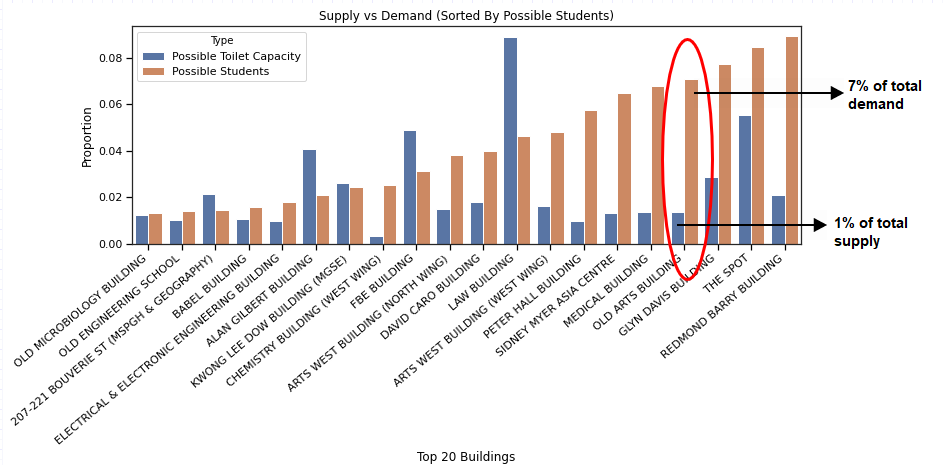
\includegraphics[width=10cm,keepaspectratio=true]{resources/images/spatial-tr/old.PNG}
% \caption{Supply vs Demand Problem in Old Arts Building}
% \label{fig:old}
% \end{figure}

% \begin{itemize}
%     \item \textbf{Best nearby buildings with no preference:}
%     As given in the appendix Table \ref{appendix:old}, a student needs to walk just \texttt{2.59} meters from Old Arts Building to use the toilet facilities with adequate supply of the mentioned facilities. The results also suggests a relaxing parameter ($\delta$) of \texttt{0} meters so that the students can do not miss out on a high rewarding building. Using these constraints,it suggest that \texttt{OLD PHYSICS BUILDING (128)} is the most rewarding building with the cost of \texttt{2.59} meters followed by \texttt{BioSciences 5 Building (194)} with cost \texttt{90.05} meters and followed by \texttt{Walter Boas (163) ,Baldwin Spencer (113), Dough McDonell (168)} Buildings with cost \texttt{157.46,184.12,275.39} meters respectively, as shown in Figure \ref{fig:o}
% \begin{figure}[H]
% \begin{subfigure}{.5\textwidth}
% \centering
%   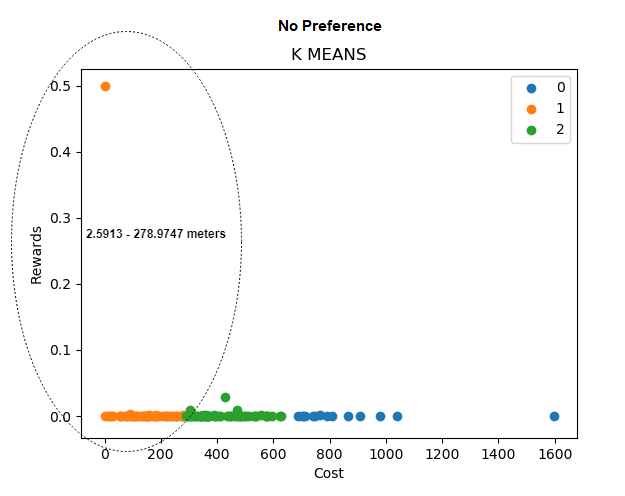
\includegraphics[width=8cm]{resources/images/spatial-tr/149plot.png}
% \end{subfigure}%
% \begin{subfigure}{.5\textwidth}
%   \centering
%   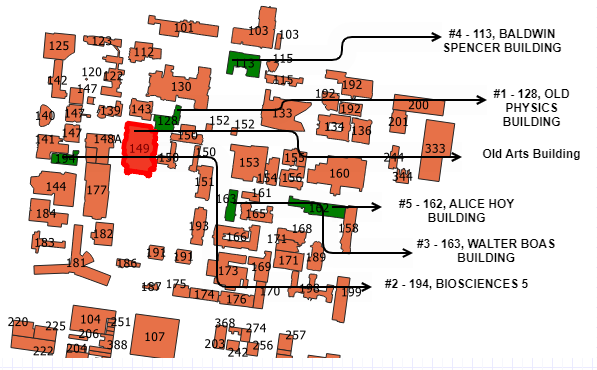
\includegraphics[width=8cm]{resources/images/spatial-tr/old1.PNG}
% \end{subfigure}
% \caption{Best rewarding cluster (left) and 3 most optimal buildings from Old Arts Building (right)}
% \label{fig:o}
% \end{figure}
    
% \item \textbf{Best nearby buildings under COVID-19 Strict Lockdown:} As given in the appendix Table \ref{appendix:old} with COVID-19 strict factor, a student should be willing to walk \texttt{2.59} meters from the mentioned building to be able to get to the buildings having an adequate supply of toilet facilities. A relaxation parameter ($\delta$) of 
% \texttt{276.32} meters could help a student to find a high rewarding building. Using the results mentioned in the table, 
% it is seen that \texttt{Alan Gilbert Building (104)} has the highest reward with \texttt{278.91} meters as the cost, 
% followed by \texttt{Glyn Davis (133), Redmond Barry (115), 
% McDonell (168)} buildings respectively with costs 
% \texttt{211.92,257.12,243.51,
% 275.39} meters.
    
% \item \textbf{Best nearby buildings with Good Toilet Room Conditions:}
% In the appendix Table \ref{appendix:old}, we have Room condition as one of the factors with its budget and relaxing budgets. Using this data, we suggest that a student should walk at least \texttt{13.22} meters to get to the rewarding building and the relaxing parameter would get a student to an even more rewarding building if a student decides to walk \texttt{147.1} meters from the current building.The most rewarding building is \texttt{Old Physics Building (128)} with cost as  \texttt{2.59} and followed by \texttt{Baldwin Spencer (113), Biosciences 5 (194) , Biosciences 4 (147) ,Biosciences 4 (147)} buildings in order with their costs \texttt{184.12,90.05,97.66,75.17} meters.

% \item \textbf{Best nearby buildings with High Capacity:} As shown in the Appendix Table \ref{appendix:old} with high capacity factor, a student can easily find high supply of toilets providing buildings from Old Arts building within the budget of \texttt{2.59 metres}. Using these constraints, we again suggest \texttt{Old Physics Buildings (128)} as the most rewarding building with the cost of \texttt{2.59 metres} followed by \texttt{Walter Boas (MSHS) (163)} with \texttt{157.46 metres} and \texttt{Biosciences 5 (194)} with \texttt{90.05 metres}.

% \item \textbf{Best nearby buildings with other factors:} In the appendix Table \ref{appendix:old}, we have also shown other factors such as finding toilet rooms with easy availability with their budgets and relaxing budgets. Using those constraints, we suggest that \texttt{Old Physics Building (128) - 2.59 metres} is the most rewarding building for finding toilets which are easily available.

% The results of some of the above discussed factors are summarized below using clustering diagrams.
% \end{itemize}

% \begin{figure}[H]
% \centering
% \begin{subfigure}[b]{0.30\textwidth}
%   \centering
%   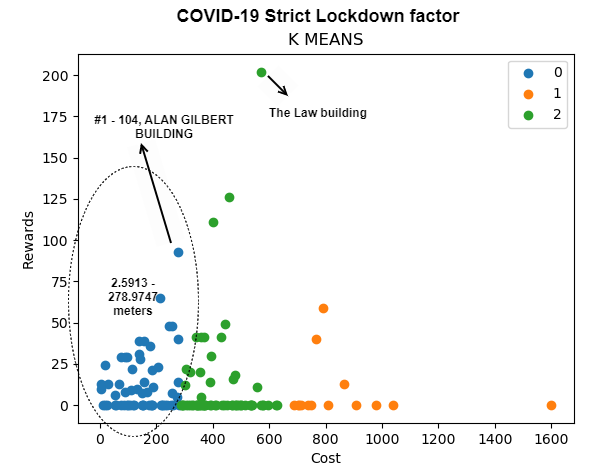
\includegraphics[width=5.5cm,keepaspectratio=true]{resources/images/spatial-tr/149_covidplot.png}
% \end{subfigure}
% \begin{subfigure}[b]{0.30\textwidth}
%   \centering
%   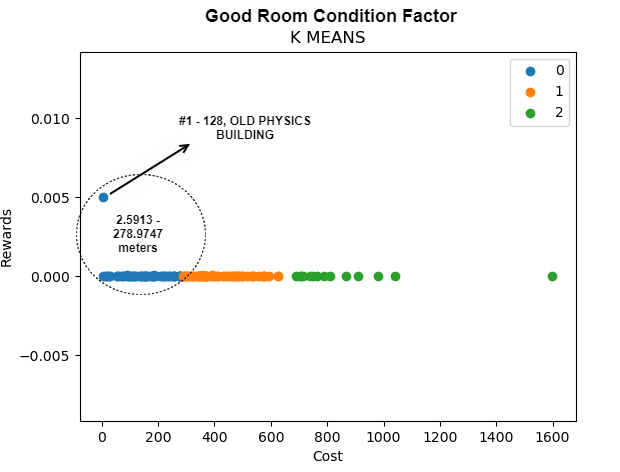
\includegraphics[width=5.5cm,keepaspectratio=true]{resources/images/spatial-tr/149_roomplot.png}
% \end{subfigure}
% \begin{subfigure}[b]{0.30\textwidth}
%   \centering
%   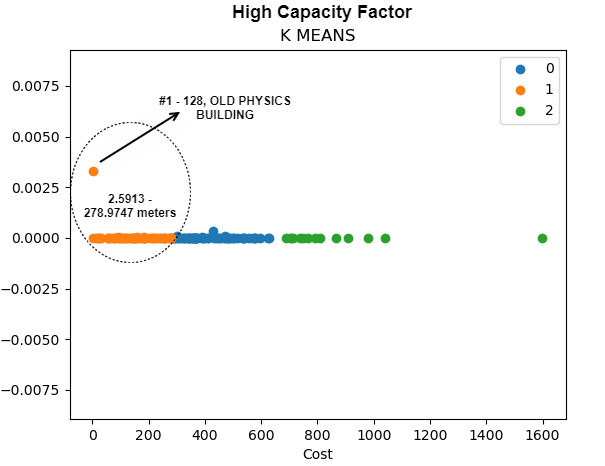
\includegraphics[width=5.5cm,keepaspectratio=true]{resources/images/spatial-tr/149_highplot.png}
% \end{subfigure}
% \caption{Best rewarding clusters of nearby buildings from Old Arts Building based on different factors}
% \label{fig:old_factors}
% \end{figure}

% \paragraph{Medical Building (Parkville Campus)}
% \begin{figure}[H]
% \centering
% 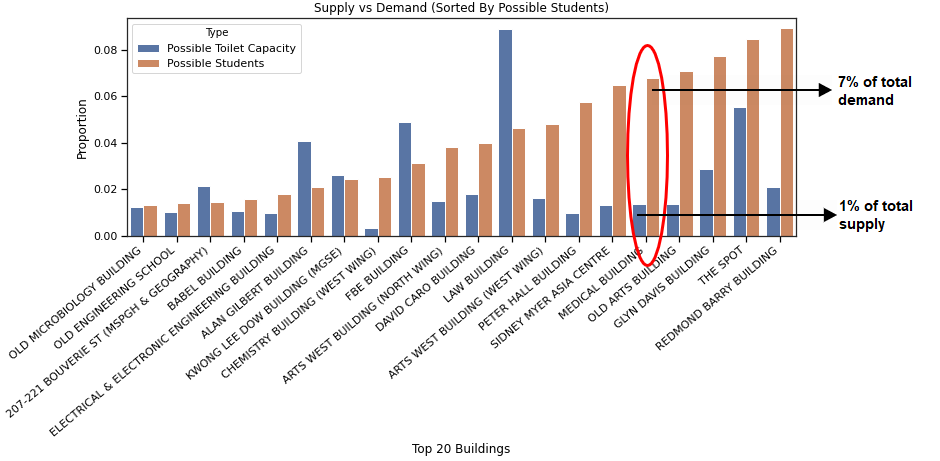
\includegraphics[width=10cm,keepaspectratio=true]{resources/images/spatial-tr/med.PNG}
% \caption{Supply vs Demand Problem in Medical Building}
% \label{fig:med}
% \end{figure}

% \begin{itemize}
%     \item \textbf{Best nearby buildings with no preference:}
%     As given in the appendix Table \ref{appendix:med}, a student needs to walk just \texttt{14.18} meters from Medical Building to use the toilet facilities with adequate supply of the mentioned facilities. The results also suggests a relaxing parameter ($\delta$) of \texttt{227.4} meters so that the students can do not miss out on a high rewarding building. Using these constraints,it suggest that \texttt{OLD PHYSICS BUILDING (128)} is the most rewarding building with the cost of \texttt{241.58} meters followed by \texttt{BioSciences 5 Building (194)} with cost \texttt{119.38} meters and followed by \texttt{200 Berkeley St(260) ,208-210 Berkeley St (204),780 Elizabeth St (220)} Buildings with cost \texttt{158.54,129.08,96.54} meters respectively, as shown in Figure \ref{fig:m}
    
% \begin{figure}[H]
% \begin{subfigure}{.5\textwidth}
% \centering
%   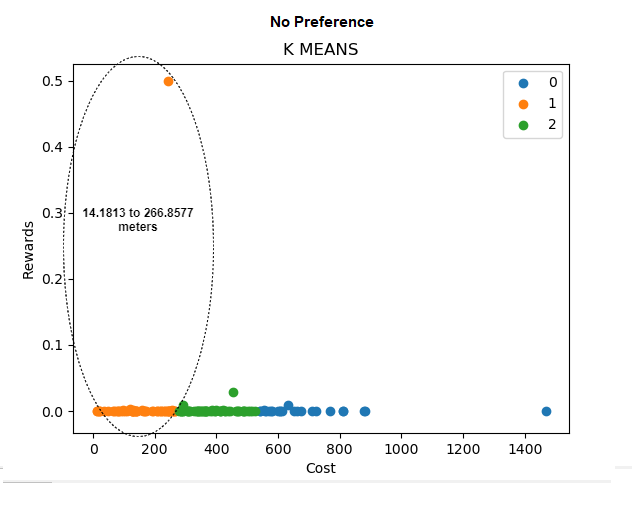
\includegraphics[width=8cm]{resources/images/spatial-tr/181plot.png}
% \end{subfigure}%
% \begin{subfigure}{.5\textwidth}
%   \centering
%   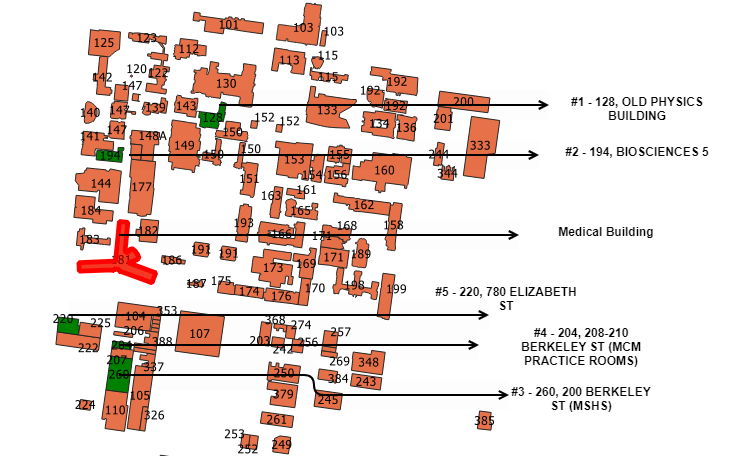
\includegraphics[width=8cm]{resources/images/spatial-tr/med1.PNG}
% \end{subfigure}
% \caption{Best rewarding cluster (left) and 3 most optimal buildings from Medical Building (right)}
% \label{fig:m}
% \end{figure}
    
% \item \textbf{Best nearby buildings under COVID-19 Strict Lockdown:} As given in the appendix Table \ref{appendix:med} with COVID-19 strict factor, a student should be willing to walk \texttt{14.18} meters from the mentioned building to be able to get to the buildings having an adequate supply of toilet facilities. A relaxation parameter ($\delta$) of \texttt{213.01} meters could help a student to find a high rewarding building. Using the results mentioned in the table, it is seen that \texttt{The Spot Building (110)} has the highest reward with \texttt{227.19} meters as the cost, followed by \texttt{The Spot (110), The FBE (105), Alan Gilbert(104) , John Medley(191)} buildings respectively with costs \texttt{169.49,47.7,83.6} meters.
    
% \item \textbf{Best nearby buildings with Excellent Toilet Room Conditions:}
% In the appendix Table \ref{appendix:med}, we have Room condition as one of the factors with its budget and relaxing budgets. Using this data, we suggest that a student should walk at least \texttt{14.18} meters to get to the rewarding building and the relaxing parameter would get a student to an even more rewarding building if a student decides to walk ($\delta$) \texttt{227.4} meters from the current building.The most rewarding building is \texttt{Old Physics Building (128)} with cost as  \texttt{241.58} meters and followed by \texttt{Alan Gilbert (104), The FBE (105), The Spot (110), John Medley (192)} buildings in order 
% with their costs \texttt{47.7,169.49,227.19,83.6} meters.

% \item \textbf{Best nearby buildings with High Capacity:} As shown in the Appendix Table \ref{appendix:med} with high capacity factor, a student can easily find high supply of toilets providing buildings from Medical building within the budget of \texttt{14.1813 metres}. Using these constraints, we again suggest \texttt{Old Physics Buildings (128)} as the most rewarding building with the cost of \texttt{241.58 metres} followed by \texttt{200 Berkeley St (MSHS) (260)} with \texttt{158.54 metres} and \texttt{Biosciences 5 (194)} with \texttt{119.38 metres}.

% \item \textbf{Best nearby buildings with other factors:} In the appendix Table \ref{appendix:med}, we have also shown other factors such as finding toilet rooms with easy availability with their budgets and relaxing budgets. Using those constraints, we suggest that \texttt{Old Physics Building (128) - 241.58 metres} is the most rewarding building for toilets with high capacity and for finding toilets which are easily available.

% The results of some of the above discussed factors are summarized below using clustering diagrams.
% \end{itemize}
% \begin{figure}[H]
% \centering
% \begin{subfigure}[b]{0.30\textwidth}
%   \centering
%   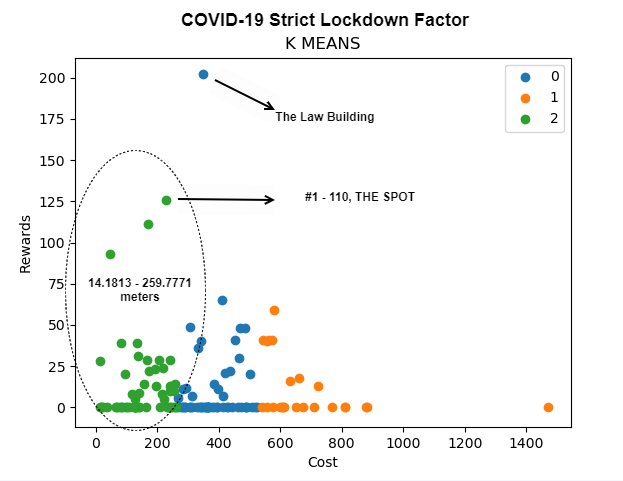
\includegraphics[width=5.5cm,keepaspectratio=true]{resources/images/spatial-tr/181_covidplot.png}
% \end{subfigure}
% \begin{subfigure}[b]{0.30\textwidth}
%   \centering
%   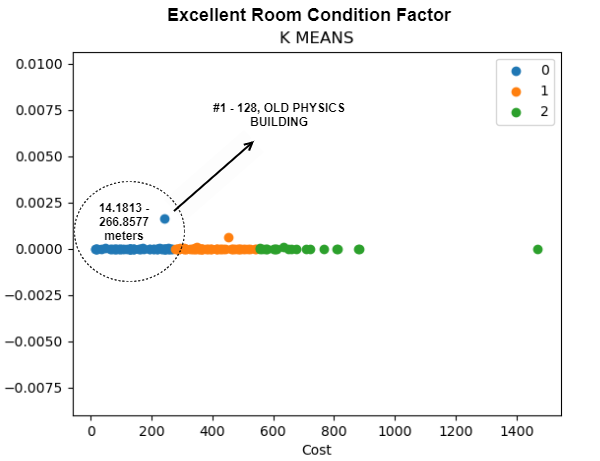
\includegraphics[width=5.5cm,keepaspectratio=true]{resources/images/spatial-tr/181_roomplot.png}
% \end{subfigure}
% \begin{subfigure}[b]{0.30\textwidth}
%   \centering
%   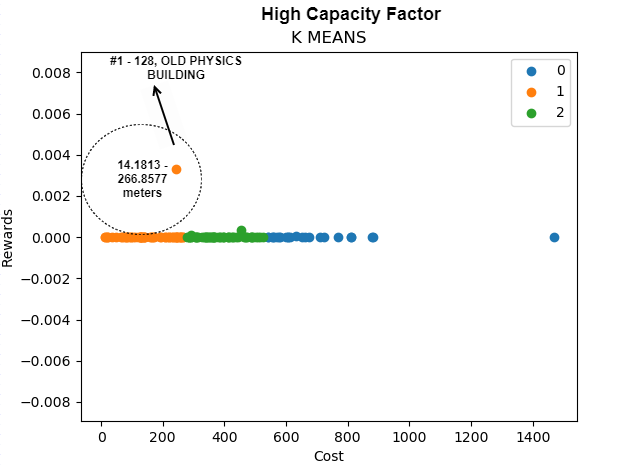
\includegraphics[width=5.5cm,keepaspectratio=true]{resources/images/spatial-tr/181_highplot.png}
% \end{subfigure}
% \caption{Best rewarding clusters of nearby buildings from Medical Building based on different factors}
% \label{fig:med_factors}
% \end{figure}

\paragraph{The Spot Building (Parkville Campus)}
\begin{figure}[H]
\centering
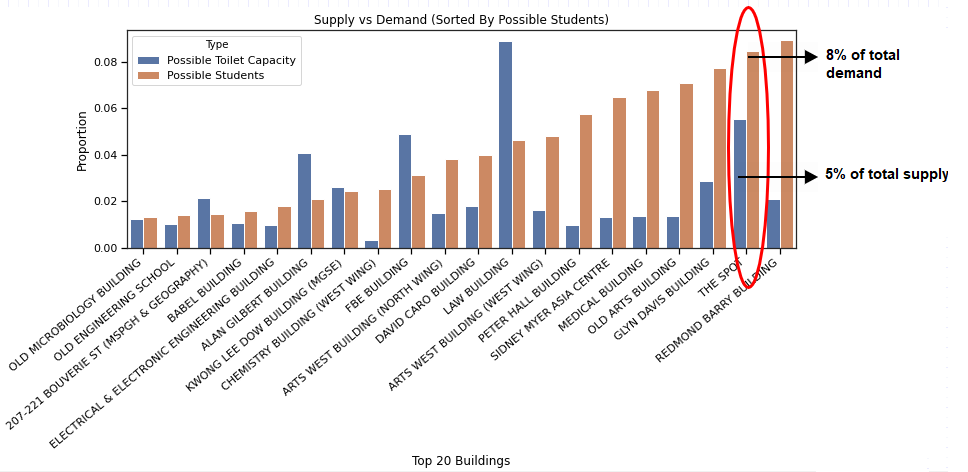
\includegraphics[width=10cm,keepaspectratio=true]{resources/images/spatial-tr/spot.PNG}
\caption{Supply vs Demand Problem in The Spot Building}
\label{fig:spot}
\end{figure}

\begin{itemize}
    \item \textbf{Best nearby buildings with no preference:}
    As given in the appendix Table \ref{appendix:spot}, a student needs to walk just \texttt{356.38} meters from The Spot Building to use the toilet facilities with an adequate supply of the mentioned facilities. The results also suggest a relaxing parameter ($\delta$) of \texttt{199.29} meters so that the students can do not miss out on a high rewarding building. Using these constraints, it suggests that \texttt{OLD PHYSICS BUILDING (128)} is the most rewarding building with the cost of \texttt{555.68} meters, as shown in Figure \ref{fig:s}.
    % followed by \texttt{757 Swanston St(STOP 1) (199)} with cost \texttt{525.28} meters and followed by \texttt{Mechanical (170), Biosciences 4 (194), 200 Berkeley St (260)} Buildings with cost \texttt{386.32,460.05,0} meters respectively
    
    \begin{figure}[H]
\begin{subfigure}{.5\textwidth}
\centering
  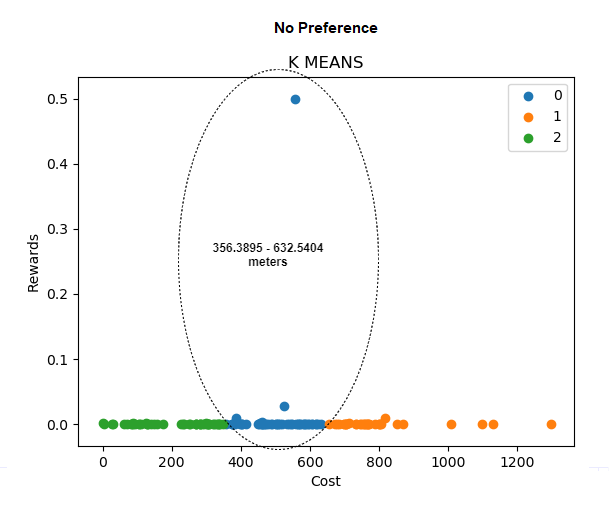
\includegraphics[width=8cm]{resources/images/spatial-tr/110plot.png}
\end{subfigure}%
\begin{subfigure}{.5\textwidth}
  \centering
  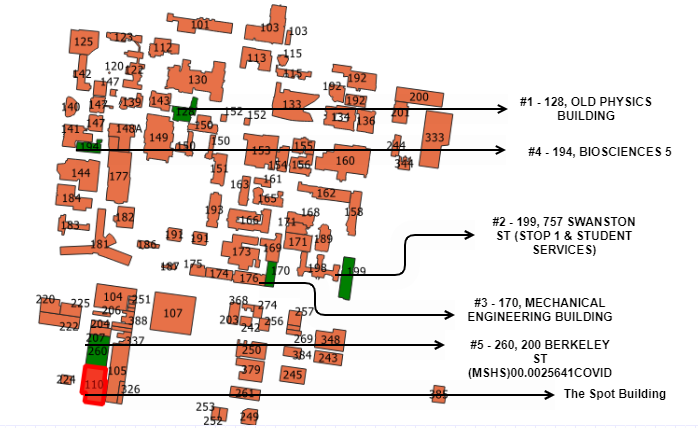
\includegraphics[width=8cm]{resources/images/spatial-tr/spot1.PNG}
\end{subfigure}
\caption{Best rewarding cluster (left) and 3 most optimal buildings from The Spot Building (right)}
\label{fig:s}
\end{figure}
    
\item \textbf{Best nearby buildings under COVID-19 Strict Lockdown:} As given in the appendix Table \ref{appendix:spot} with COVID-19 strict factor, a student should be willing to walk at least \texttt{348} meters from the mentioned building to be able to get to the buildings having an adequate supply of toilet facilities. Using the above budget, \texttt{The Law Building} is the most rewarding building with the cost of 86.79 metres.
    
% \item \textbf{Best nearby buildings with Excellent Toilet Room Conditions:}
% In the appendix Table \ref{appendix:spot},we have Room condition as one of the factors with its budget and relaxing budgets. Using this data, we suggest that a student should walk at least \texttt{356.38} meters to get to the rewarding building and the relaxing parameter would get a student to an even more rewarding building if a students decides to walk ($\delta$) \texttt{199.29} meters from the current building.The most rewarding building is \texttt{Old Physics Building (128)} with cost as  \texttt{555.68} meters and followed by \texttt{757 Swanston St(STOP 1) (199),The Law (106), Mechanical Engineering (170),
% Alan Gilbert (104)} buildings in order with their costs \texttt{525.28,86.79,386.32,128.96} meters.

% \item \textbf{Best nearby buildings with Easy Availability:} As shown in the Appendix Table \ref{appendix:spot} with easy available factor, a student can easily find high supply of toilets providing buildings from The Spot building within the budget of \texttt{357 metres}. Using these constraints, we again suggest \texttt{Old Physics Buildings (128)} as the most rewarding building with the cost of \texttt{555.68 metres} followed by \texttt{757 Swanston St(STOP 1) (199)} with \texttt{525.28 metres} and \texttt{Mechanical Engineering (170)} with \texttt{386.32 metres}.

\item \textbf{Best nearby buildings with other factors:} In the appendix Table \ref{appendix:med}, we have also shown other factors such as finding toilet rooms with high capacity with their budgets and relaxing budgets. Using those constraints, we suggest that \texttt{Old Physics Building (128) - 555.68 meters} is the most rewarding building for toilets with high capacity. The \texttt{Law Building (106)} has the highest reward with \texttt{86.79} meters as the cost for excellent toilet room condition and \texttt{The Spot building} within the budget of \texttt{357} metres.

The results of some of the above-discussed factors are summarized below using clustering diagrams.

\begin{figure}[H]
\centering
\begin{subfigure}[b]{0.30\textwidth}
  \centering
  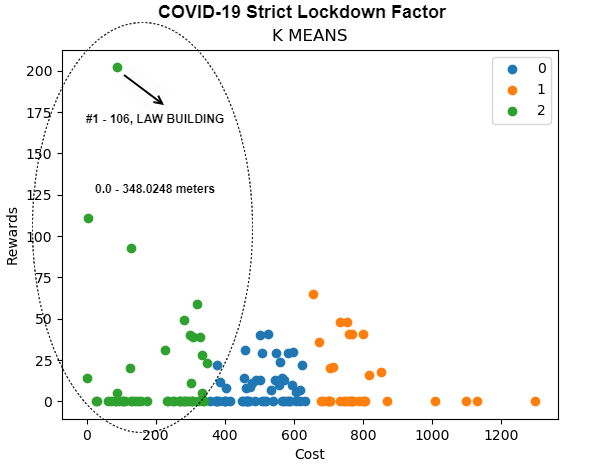
\includegraphics[width=5.5cm,keepaspectratio=true]{resources/images/spatial-tr/110_covidplot.png}
\end{subfigure}
\begin{subfigure}[b]{0.30\textwidth}
  \centering
  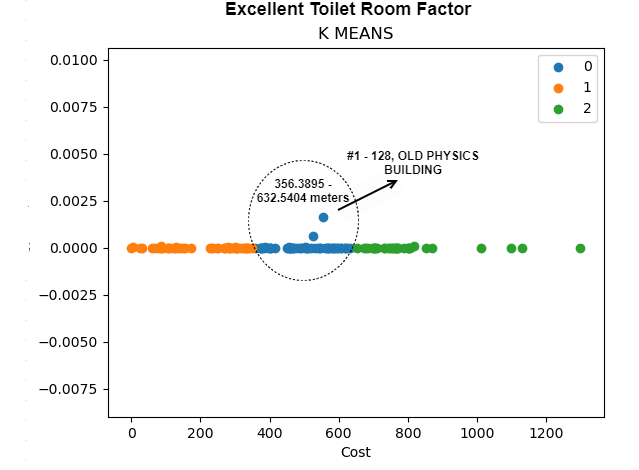
\includegraphics[width=5.5cm,keepaspectratio=true]{resources/images/spatial-tr/110_roomplot.png}
\end{subfigure}
\begin{subfigure}[b]{0.30\textwidth}
  \centering
  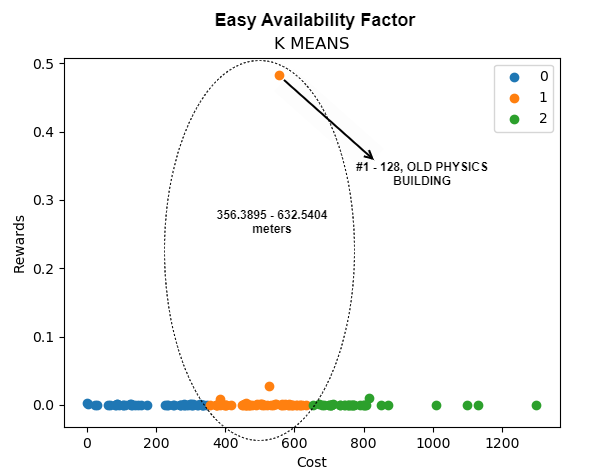
\includegraphics[width=5.5cm,keepaspectratio=true]{resources/images/spatial-tr/110_easyplot.png}
\end{subfigure}
\caption{Best rewarding clusters of nearby buildings from The Spot Building based on different factors}
\label{fig:spot_factors}
\end{figure}
\end{itemize}

\paragraph{Ian Potter Southbank Centre Building (Southbank Campus)}
\begin{figure}[H]
\centering
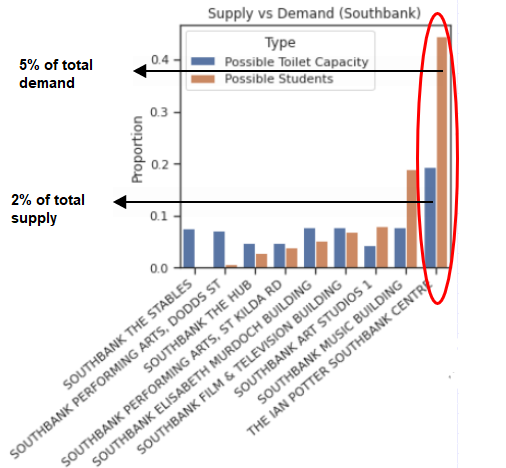
\includegraphics[width=10cm,keepaspectratio=true]{resources/images/spatial-tr/ian.PNG}
\caption{Supply vs Demand Problem in The Ian Potter Southbank Centre Building}
\label{fig:ian}
\end{figure}

\begin{itemize}
    \item \textbf{Best nearby buildings with no preference:}
    As given in the appendix Table \ref{appendix:sth-ian}, a student needs to walk just at least \texttt{114} meters from  Ian Potter Southbank Centre Building to use the toilet facilities with adequate supply of the mentioned facilities. Using the above budget, it suggests that \texttt{The Stables (873)} is the most rewarding building with the cost of \texttt{97.82} meters, as shown in Figure \ref{fig:i}
    
     \begin{figure}[H]
\begin{subfigure}{.5\textwidth}
\centering
  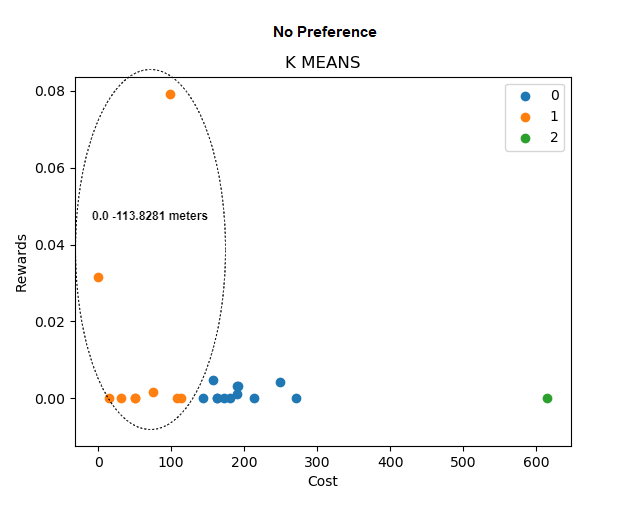
\includegraphics[width=8cm]{resources/images/spatial-tr/880plot.png}
\end{subfigure}%
\begin{subfigure}{.5\textwidth}
  \centering
  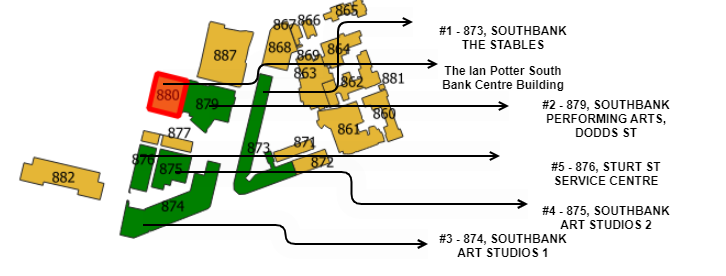
\includegraphics[width=8cm]{resources/images/spatial-tr/ian1.PNG}
\end{subfigure}
\caption{Best rewarding cluster (left) and 3 most optimal buildings from The Ian Potter Southbank Centre Building (right)}
\label{fig:i}
\end{figure}
    
\item \textbf{Best nearby buildings under COVID-19 Strict Lockdown:} As given in the appendix Table \ref{appendix:sth-ian} with COVID-19 strict factor, a student should be willing to walk \texttt{143.56} meters from the mentioned building to be able to get to the buildings having an adequate supply of toilet facilities. A relaxation parameter ($\delta$) of \texttt{46.1} meters could help a student to find a high rewarding building. Using the results mentioned in the table, it is seen that the \texttt{Music Building (862)} has the highest reward with \texttt{189.67} meters as the cost.

% \item \textbf{Best nearby buildings with Easy Availability:} As shown in the Appendix Table \ref{appendix:sth-ian} with easy available factor, a student can easily find high supply of toilets providing buildings from The Ian Potter Southbank Centre building within the budget of \texttt{0 metres} and relaxation parameter of  \texttt{98 meters}. Using these constraints, we again suggest \texttt{The Stables Buildings (873)} as the most rewarding building with the cost of \texttt{97.82 metres} followed by \texttt{Performing Arts Dodds St (879)} with \texttt{0 metres} and \texttt{Art Studio 1 (874)} with \texttt{75.3 metres}.

% \item \textbf{Best nearby buildings with Good Condition Rooms:} As shown in the Appendix Table \ref{appendix:sth-ian} with good room condition factor, a student can easily find high supply of toilets providing buildings from The Ian Potter Southbank Centre building within the budget of \texttt{0 metres} and relaxation parameter of  \texttt{98 meters}. Using these constraints, we again suggest \texttt{The Stables Buildings (873)} as the most rewarding building with the cost of \texttt{97.82 metres} followed by \texttt{Performing Arts Dodds St (879)} with \texttt{0 metres} and \texttt{Art Studio 1 (874)} with \texttt{75.3 metres}.

\item \textbf{Best nearby buildings with other factors:} In the appendix Table \ref{appendix:sth-ian}, we have also shown other factors such as finding toilet rooms with high capacity, good toilet condition, with their budgets and relaxing budgets. Using those constraints, we suggest that \texttt{The Stables Buildings (873) - 97.82 meters} is the most rewarding building for toilets with high capacity, easy availability, and good conditions.

The results of some of the above-discussed factors are summarized below using clustering diagrams.

\begin{figure}[H]
\centering
\begin{subfigure}[b]{0.30\textwidth}
  \centering
  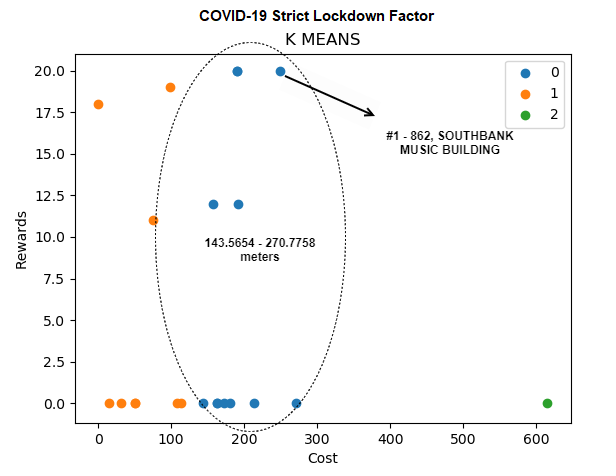
\includegraphics[width=5.5cm,keepaspectratio=true]{resources/images/spatial-tr/880_covidplot.png}
\end{subfigure}
\begin{subfigure}[b]{0.30\textwidth}
  \centering
  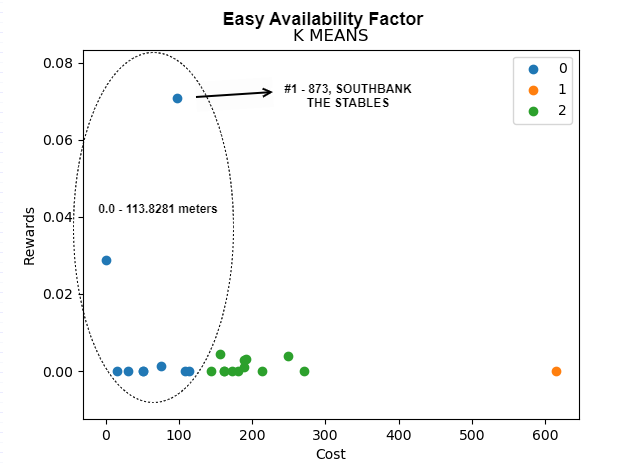
\includegraphics[width=5.5cm,keepaspectratio=true]{resources/images/spatial-tr/880_easyplot.png}
\end{subfigure}
\begin{subfigure}[b]{0.30\textwidth}
  \centering
  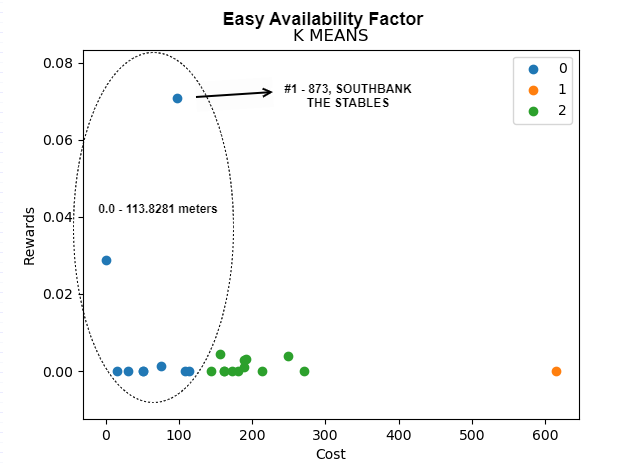
\includegraphics[width=5.5cm,keepaspectratio=true]{resources/images/spatial-tr/880_easyplot.png}
\end{subfigure}
\caption{Best rewarding clusters of nearby buildings from The Ian Potter Southbank Centre Building based on different factors}
\label{fig:ian_factors}
\end{figure}
\end{itemize}

% \paragraph{Werribee Pathology Building (Werribee Campus)}
% \begin{figure}[H]
% \centering
% 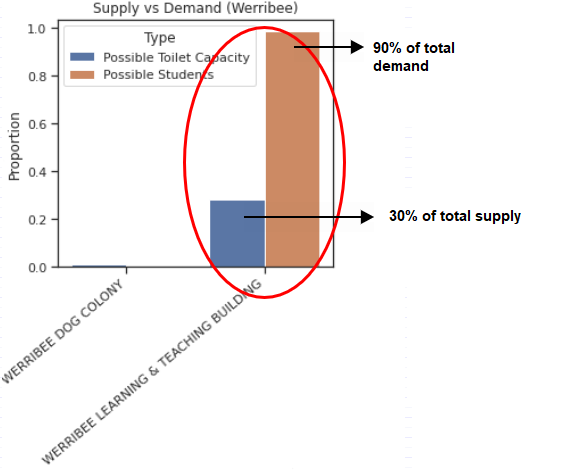
\includegraphics[width=10cm,keepaspectratio=true]{resources/images/spatial-tr/werl.PNG}
% \caption{Supply vs Demand Problem in The Werribee Pathology Building}
% \label{fig:wer}
% \end{figure}

% \begin{itemize}
%     \item \textbf{Best nearby buildings with no preference:}
%     As given in the appendix Table \ref{appendix:wer-path}, a student needs to walk just \texttt{113.35} meters from Pathology Building to use the toilet facilities with an adequate supply of the mentioned facilities. The results also suggest a relaxing parameter ($\delta$) of \texttt{40.15} meters so that the students can do not miss out on a high rewarding building. Using these constraints,it suggest that \texttt{Dog Colony (420)} is the most rewarding building with the cost of \texttt{153.5} meters followed by \texttt{The Learning and Teaching (418)} with cost \texttt{33.68} meters, as shown in Figure \ref{fig:w}
    
%  \begin{figure}[H]
% \begin{subfigure}{.5\textwidth}
% \centering
%   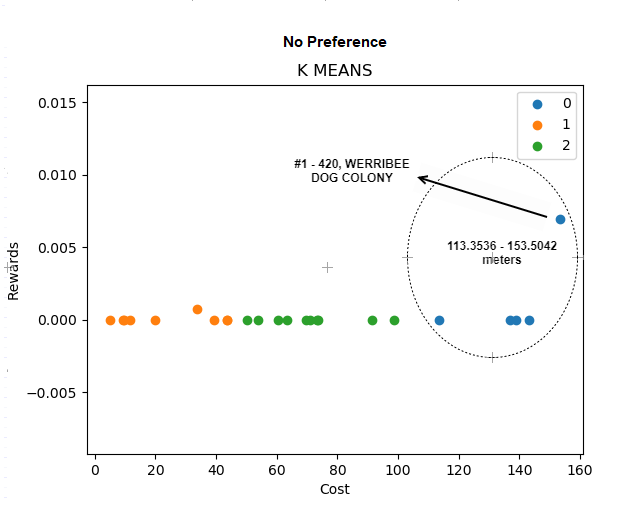
\includegraphics[width=8cm]{resources/images/spatial-tr/416plot.png}
% \end{subfigure}%
% \begin{subfigure}{.5\textwidth}
%   \centering
%   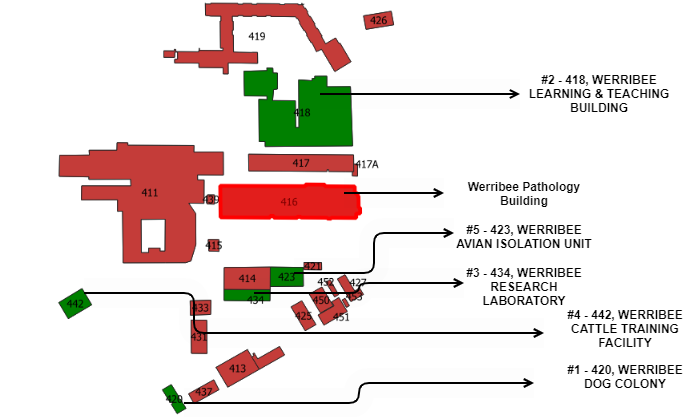
\includegraphics[width=8cm]{resources/images/spatial-tr/416_1.PNG}
% \end{subfigure}
% \caption{Best rewarding cluster (left) and 3 most optimal buildings from The Werribee Pathology Building (right)}
% \label{fig:w}
% \end{figure}
    
% \item \textbf{Best nearby buildings under COVID-19 Strict Lockdown:} As given in the appendix Table \ref{appendix:wer-path} with COVID-19 strict factor, 
% a student should be willing to walk \texttt{5.12} 
% meters from the mentioned building to be able 
% to get to the buildings having an adequate supply of toilet 
% facilities. A relaxation parameter ($\delta$) of \texttt{28.56} meters could help a student to find a high rewarding building. 
% Using the results mentioned in the table, it is seen that \texttt{The Learning and Teaching (418)} has the 
% the highest reward with \texttt{33.68} meters as the cost.

% \item \textbf{Best nearby building with Excellent Toilet Rooms Condition:}
% In the appendix Table \ref{appendix:wer-path},we have Room condition as one of the factors with its budget and relaxing budgets. Using this data, we suggest that a student should walk at least \texttt{114} meters to get to the rewarding building and the relaxing parameter would get a student to an even more rewarding building if a students decides to walk \texttt{24} meters from the current building.The most rewarding building is \texttt{Research Laboratory (434)} and followed by \texttt{Cattle Training Facility (442), Aviation Isolation Unit (434) buildings} in order with costs \texttt{0,0,0} meters.

% \item \textbf{Best nearby building with other factors:}
%  In the appendix Table \ref{appendix:wer-path}, we have also shown other factors such as finding toilet rooms with high capacity and easy availability with their budgets and relaxing budgets. Using those constraints, we suggest that \texttt{Dog Colony Building (420) - 153.5 metres} is the most rewarding building for toilets with high capacity and easy availability.

% The results of some of the above discussed factors are summarized below using clustering diagrams.


% \begin{figure}[H]
% \centering
% \begin{subfigure}[b]{0.30\textwidth}
%   \centering
%   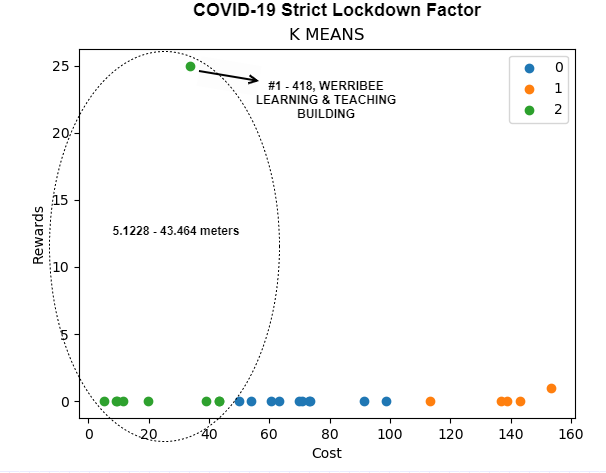
\includegraphics[width=5.5cm,keepaspectratio=true]{resources/images/spatial-tr/416_covidplot.png}
% \end{subfigure}
% \begin{subfigure}[b]{0.30\textwidth}
%   \centering
%   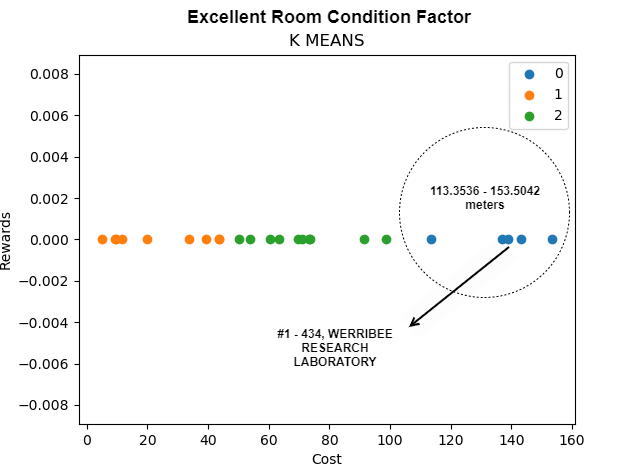
\includegraphics[width=5.5cm,keepaspectratio=true]{resources/images/spatial-tr/416_roomplot.png}
% \end{subfigure}
% \begin{subfigure}[b]{0.30\textwidth}
%   \centering
%   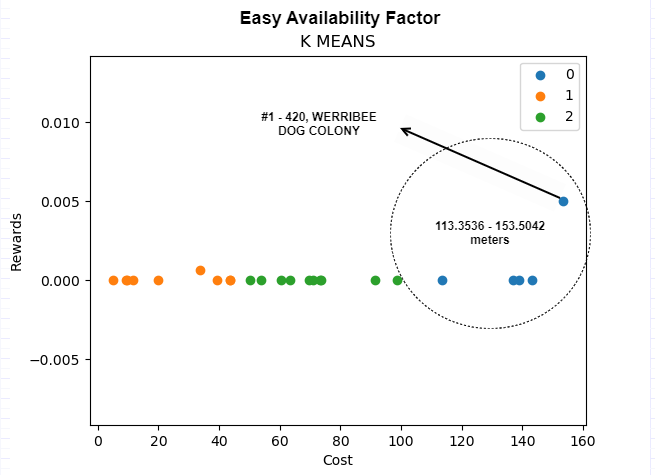
\includegraphics[width=5.5cm,keepaspectratio=true]{resources/images/spatial-tr/416_easyplot.png}
% \end{subfigure}
% \caption{Best rewarding clusters of nearby buildings from The Werribee Pathology Building based on different factors}
% \label{fig:pat_factors}
% \end{figure}
% \end{itemize}
